\documentclass[a4paper,12pt,french] {article}

\usepackage[sujet]{../../../Style}

\fancyhead[L]{08/12/2021}
\fancyhead[C]{\textbf{DS3 : Suites - Généralités}}
\fancyhead[R]{\premiere ST2S 2}

\renewcommand{\baselinestretch}{1.35}

\begin{document}

\rem[black]{L'usage de la calculatrice est autorisé. La propreté et l'orthographe seront prises en compte. Tout le devoir peut être fait sur le sujet.}

Nom: \hfill Prénom: \hfill \

\begin{exercice} \
\compohaut[0.4]{
\begin{enumerate}
\item Soit $u$ une suite dont le premier terme est $u_{24}$. Donner:
\begin{itemize}
\item Son troisième terme: \dotfill
\item Son septième terme: \dotfill
\item Son dixième terme: \dotfill
\end{itemize}
\end{enumerate}
}
{
\begin{enumerate}[start=2]
\item On se donne la suite $v$ définie pour tout $n \in \N$ par $v_n=2n^2-11$. Compléter:
\begin{itemize}
\item $v_0=$\dotfill
\item $v_1=$\dotfill
\item $v_2=$\dotfill
\item $v_7=$\dotfill
\end{itemize}
\end{enumerate}
}
\end{exercice}

\begin{exercice} \

\begin{enumerate}
\item Compléter le schéma suivant:

\noindent 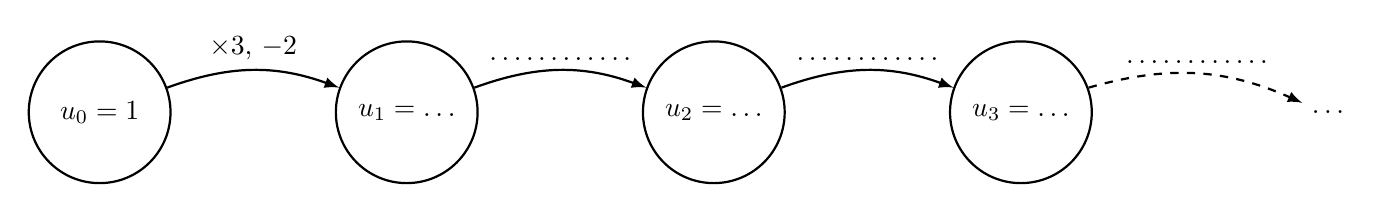
\begin{tikzpicture}[scale=1.3]
\node[draw,circle,thick, minimum size=18mm] (W0) at (-3,0) {$u_0=1$};
\node[draw,circle,thick, minimum size=18mm] (W1) at (0,0) {$u_1=\ldots$};
\node[draw,circle,thick, minimum size=18mm] (W2) at (3,0) {$u_2=\ldots$};
\node[draw,circle,thick, minimum size=18mm] (W3) at (6,0) {$u_3=\ldots$};
\node (W4) at (9,0) {$\ldots$};
\draw[->,>=latex,thick] (W0) to[bend left=20] node[midway,above]{$\times 3$, $-2$} (W1);
\draw[->,>=latex,thick] (W1) to[bend left=20] node[midway,above]{$\makebox[2cm]{\dotfill}$} (W2);
\draw[->,>=latex,thick] (W2) to[bend left=20] node[midway,above]{$\makebox[2cm]{\dotfill}$} (W3);
\draw[->,>=latex,thick,dashed] (W3) to[bend left=20] node[midway,above]{$\makebox[2cm]{\dotfill}$} (W4);
\end{tikzpicture}

\item Compléter alors la relation de récurrence suivante: $\left\{ \begin{matrix} u_0=\ldots \\ u_{n+1}= \ldots u_n \ldots \end{matrix} \right.$

\item Soit $w$ une suite telle que $w_0=3$ et pour $n \in \N$, $w_{n+1}=w_n^2-7$. Calculer:
\begin{itemize}
\item $w_1=$ \points 1
\item $w_2=$ \points 1
\item $w_3=$ \points 1
\end{itemize}
\item Vrai ou faux? La suite $w$ est décroissante. \makebox[3cm]{\dotfill}
\end{enumerate}

\end{exercice}

\begin{exercice}
On se donne la suite $u$ représentée ci-dessous:
\begin{center}
\begin{tikzpicture}[scale=\echellepgf]
\begin{axis}[
styleglobal,
%hauteurproptick,
width=0.9*\echellepgfinv*\linewidth,
xmin=0, xmax= 10,
ymin=-1.5, ymax=2.5,
xlabel={$n$},
ylabel={$u_n$},
minor x tick num=1,
minor y tick num=1,
xtick distance=1,
ytick distance=0.5,
label style= {font=\normalsize},
grid style={densely dashed,line width=0.5pt},
]
\addplot[draw=none,samples=11,domain=(0:10),mark=*] {0.1*floor(10*sqrt(x))-1.2};
\end{axis}
\end{tikzpicture}
\end{center}

\begin{enumerate}

\item Déterminer graphiquement $u_2$ et $u_9$: \dotfill
\item Emettre une conjecture concernant les variations de $u$.

\points 1

\item On définit la suite $v$ telle que pour tout $n \in \N, v_n=6n+11$.
\end{enumerate}

\compo[0.5]
{
\begin{enumerate}[label=\alph{enumi})]
\item Représenter la suite dans le repère ci-contre (pour $n$ allant de $0$ à $5$).
\item Emettre puis prouver une conjecture concernant les variations de $v$. On calculera $v_{n+1}-v_n$:

\points 5
\end{enumerate}
}
{
\begin{center}
\begin{tikzpicture}[scale=\echellepgf]
\begin{axis}[
styleglobal,
hauteurproptick,
width=0.9*\echellepgfinv*\linewidth,
xmin=0, xmax= 5.5,
ymin=0, ymax=50,
xlabel={$n$},
ylabel={$u_n$},
minor x tick num=1,
minor y tick num=1,
xtick distance=1,
ytick distance=10,
label style= {font=\normalsize}
]
\end{axis}
\end{tikzpicture}
\end{center}
}

\vspace{6mm} \setstretch{1.5}{

\hspace{3mm} \dotfill \

\hspace{3mm} \dotfill}

\end{exercice}

\begin{exercice}


\begin{enumerate}
\item La moitié de la carte d'un restaurant est composée de plats végétariens. Parmi ceux-ci, 20 $\%$ contiennent des tomates. Déterminer la proportion de plats végétariens contenant des tomates dans la carte du restaurant.

\points 4

\item Le prix d'un litre d'essence a augmenté de $15 \%$ entre janvier et avril, puis de $10 \%$ entre avril et septembre, et enfin de $20 \%$ entre septembre et décembre. Calculer son évolution globale.

\points 4

\end{enumerate}
\end{exercice}

\end{document}